\paragraph{Volumetric benchmark results.}

Figure~\ref{fig:3d_appendix_profiles} reports recognition, open-ended question answering, and report generation results. CoEvoMed leads all five M3D-VQA categories, with 80.11\% overall accuracy (11,048/13,791) and 83.06\% macro-averaged accuracy across categories; Med3DVLM-7B (Med3DVLM-Qwen-2.5-7B)~\citep{xin2025med3dvlm} reaches 79.18\% overall accuracy. These results support CoEvoMed's applicability across complementary volumetric medical tasks.

\begin{figure}[!htbp]
\centering
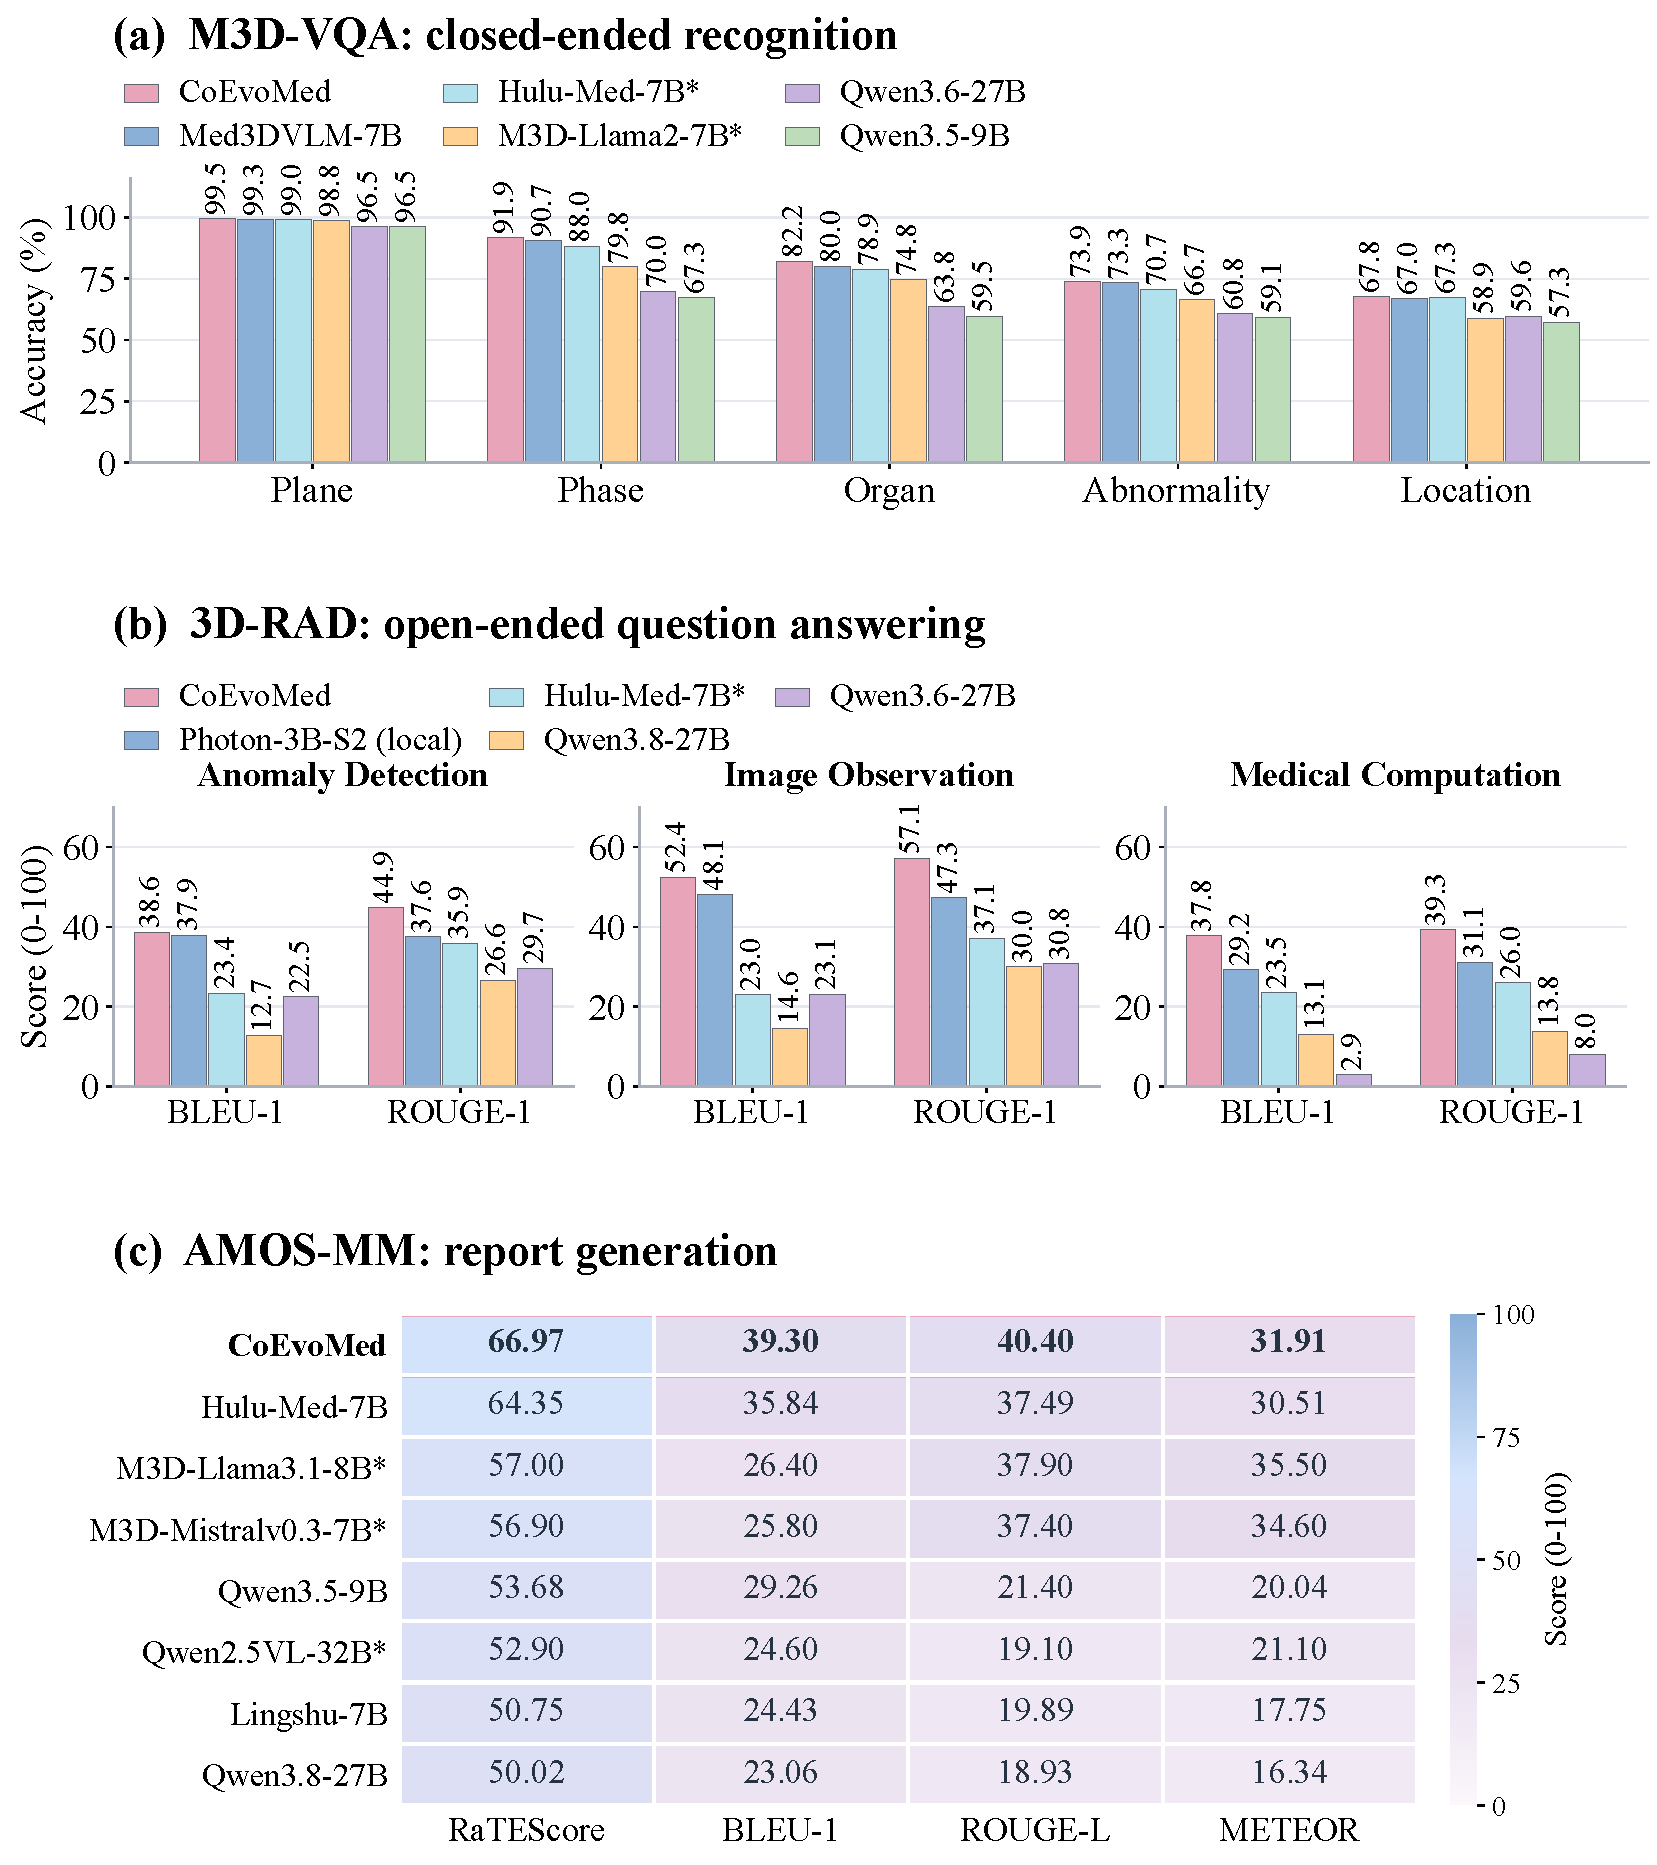
\includegraphics[width=\linewidth]{figures/three_d_appendix_profiles.pdf}
\caption{Detailed 3D benchmark profiles. (a) M3D-VQA closed-ended accuracy across five categories. (b) 3D-RAD open-ended BLEU-1 and ROUGE-1 across three tasks; Photon uses its local S2 evaluation. (c) AMOS-MM report generation metrics, with raw values and a fixed 0--100 color scale. Each panel includes CoEvoMed and the highest-ranked available baselines: five by mean category accuracy in (a), four by mean task ROUGE-1 in (b), and seven by RaTEScore in (c). All scores are scaled to 100. Asterisks mark results from \citet{jiang2025hulumed}.}
\label{fig:3d_appendix_profiles}
\end{figure}
